\documentclass{article}
\usepackage{fullpage}	
\setlength\parindent{0pt}
\everymath{\displaystyle}
\usepackage{graphicx}

\begin{document}
Quiz 9 Jason Dorweiler

1. Suppose that a biologist is studying a fixed population of gorillas. How can the biologist use a graph to encode whether pairs of gorillas have exhibited hostility toward each other? Clearly describe the meaning of the vertices and the edges.

They could use a niche overlap graph.  The book discusses the use of this type of graph to model competition between animals in an ecosystem.  For the gorillas each node would represent and individual animal and the edges would be if they have shown hostility to each other. \\



2. Consider a graph where vertices are individuals and edges are drawn between vertices of individuals who are mutual friends. Argue that the sum across all individuals of their mutual friends is an even number.\\

Since we are given that a edge represents a mutual friendship then, this will be an undirected graph.  Since it is undirected we can use the handshake theorem to prove this.\\

The sum across all individuals of their mutual friends will be $\sum_{v \in V} deg(v)$, which from the handshake theorem says that the sum of degrees of each vertex in an undirected graph is equal to 2(m) where m is the number of edges.  In our graph m is a mutual friendship and so this proves that the sum will always be even. \\

3. a) Draw a graph with 6 vertices that is bipartite. Explain why it is bipartite. b) Draw a graph with 6 vertices that is not bipartite. Explain why it is not bipartite.\\

a. This graph is bipartite because can have a two coloring with no two of the came colors being connected.  It is also a $C_{6}$ which is bipartite for even n. 

b. This graph is not bipartite because you cannot assign a two coloring with any two colors not being connected because of the internal 3 node cycles.  It is also a $W_{6}$ which are never bipartite for any value of n. 
\begin{figure}[h!]
\centering
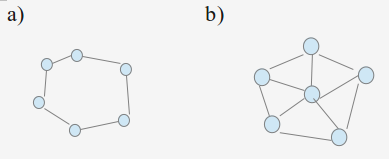
\includegraphics[width=0.5\textwidth]{quiz10pic}
\end{figure} 

4. Consider a graph G such that at least one vertex v is connected to all other vertices. Prove that G is not bipartite.
Note: remember that not all things are able to be proved, and that some things can be disproved.\\

Proof by contradiction.  Assume that graph G has a vertex v that is connected to all other verticies and is bipartite.  For a graph with $n\geq3$ verticies the vertex connecting all others will always form at least one 3 member cycle.  A bipartite graph cannot contain a three member cycle so this is a contradiction. \\

\newpage 

5. a) According to the definitions used in our book, Is it possible for a graph to have both an Euler path and Euler circuit? Explain your answer. b) Draw a directed graph involving 6 vertices that is weakly connected but not strongly connected.

a. It is not possible for a graph to have both a Euler path and Euler circuit.  A graph has a circuit if and only if all vertices have even degree. There is a path if and only if there are two vertices with an odd degree. 

\begin{figure}[h!]
\centering
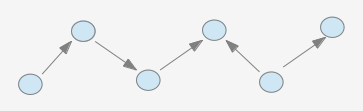
\includegraphics[width=0.5\textwidth]{quizpic2}
\end{figure} 

\end{document}



